\chapter{Kết quả thu được}
\section{Kết quả thực hiện phần cứng thực tế}
\subsection{Kết quả thiết kế phần cứng trên phần mềm}
Thực hiện sắp xếp linh kiện hợp lý trên mạch PCB hai lớp, với các linh kiện được bố trí chủ yếu ở lớp Top. Khối tạo nguồn cách ly 5V, hai port sử dụng cho Modbus RTU,
Màn hình LCD và nút nhấn đặt ở lớp Bottom.

\begin{figure}[H]
    \centering
    \begin{minipage}{0.48\textwidth}
        \centering
        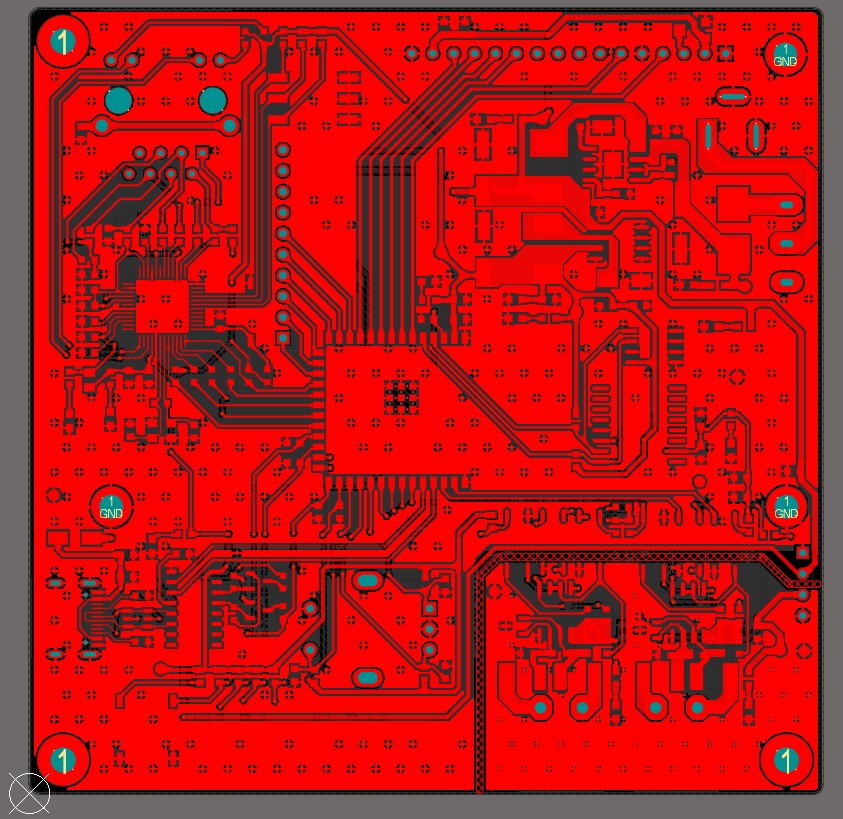
\includegraphics[width=\textwidth]{image/top_2d.png}
    \end{minipage}
    \hfill
    \begin{minipage}{0.48\textwidth}
        \centering
        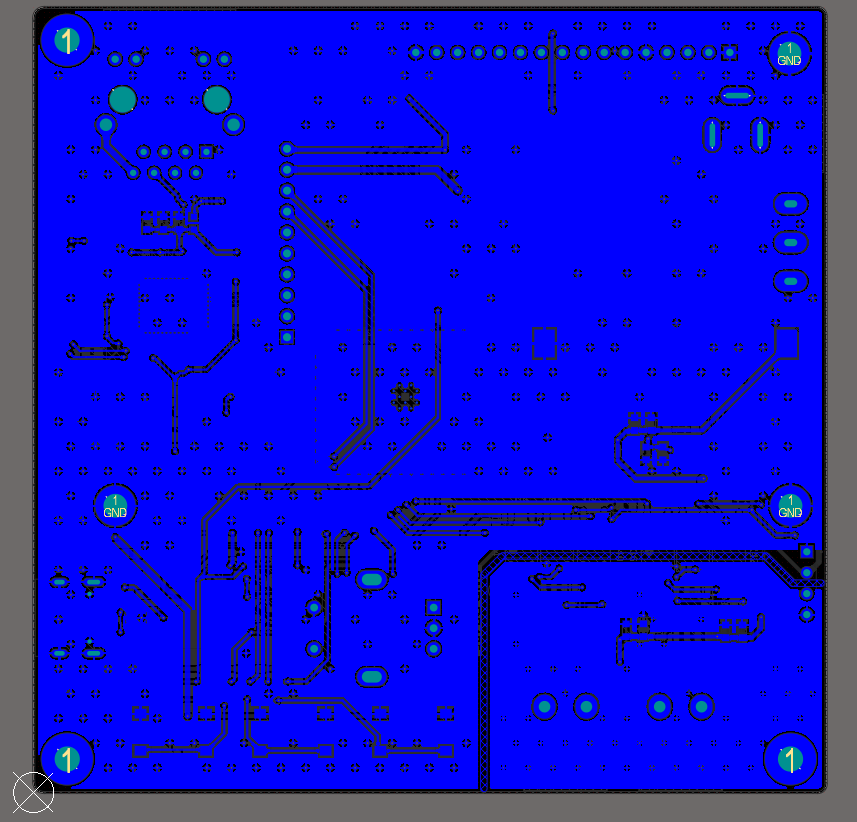
\includegraphics[width=\textwidth]{image/bottom_2d.png}
    \end{minipage}
    \caption{Hình ảnh mạch 2D sau khi đã đi dây ở lớp Top và lớp Bottom}
    \label{fig:bottom_hide_3d}
\end{figure}

\begin{figure}[H]
    \centering
    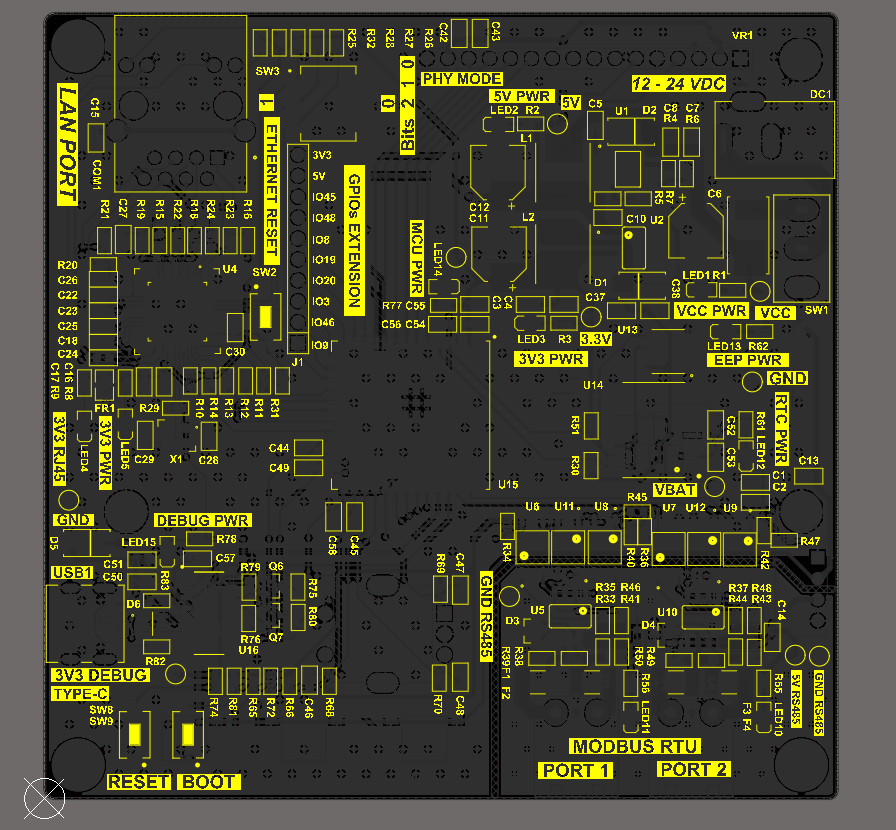
\includegraphics[width=0.6\textwidth]{image/top_layer_2d.png}
    \caption{phần đặt các ký hiệu trên bề mặt của lớp Top}
    \label{fig: top_layer_2d}
\end{figure}

\begin{figure}[H]
    \centering
    \begin{minipage}{0.48\textwidth}
        \centering
        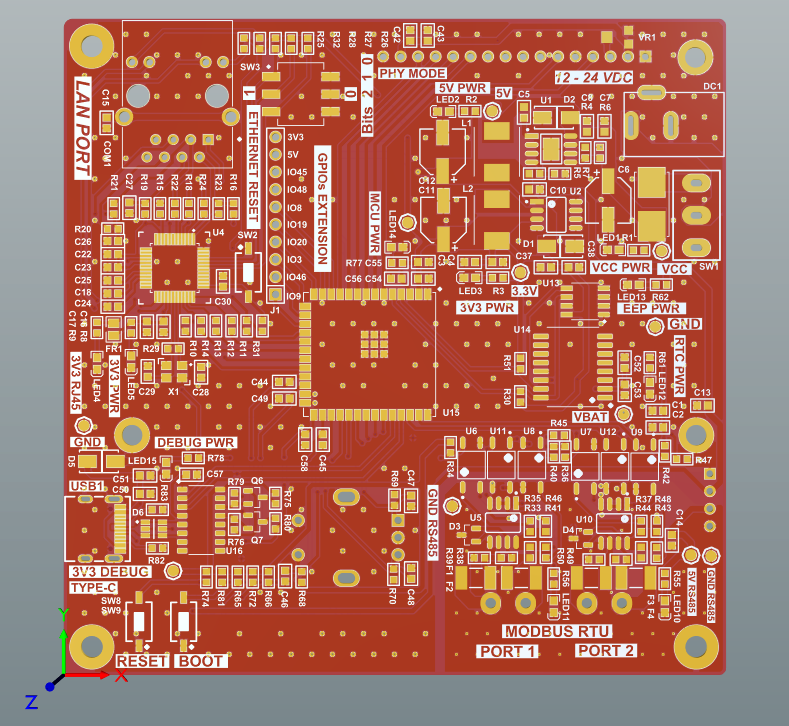
\includegraphics[width=\textwidth]{image/top_hide_3d.png}
    \end{minipage}
    \hfill
    \begin{minipage}{0.48\textwidth}
        \centering
        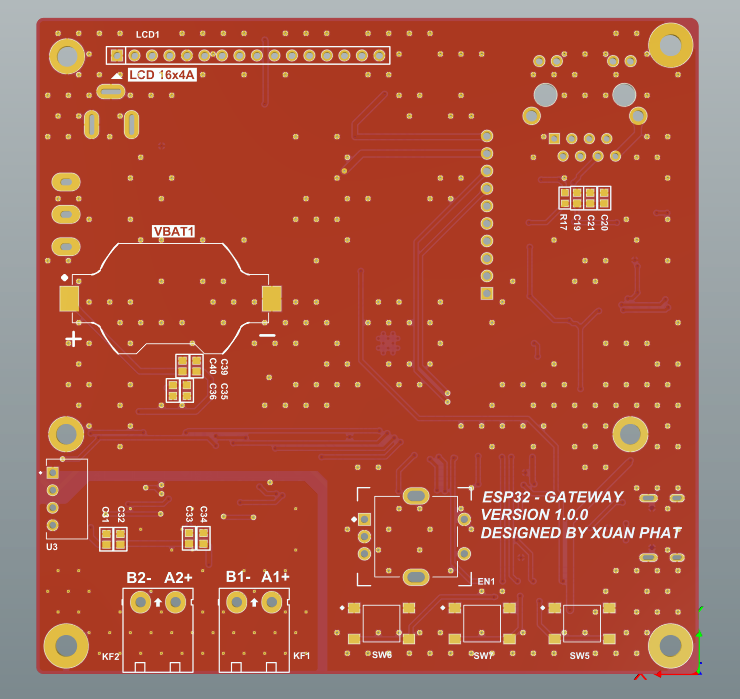
\includegraphics[width=\textwidth]{image/bottom_hide_3d.png}
    \end{minipage}
    \caption{Hình ảnh mạch 3D khi chưa đặt linh kiện của lớp Top và lớp Bottom}
    \label{fig:bottom_hide_3d}
\end{figure}

\begin{figure}[H]
    \centering
    \begin{minipage}{0.48\textwidth}
        \centering
        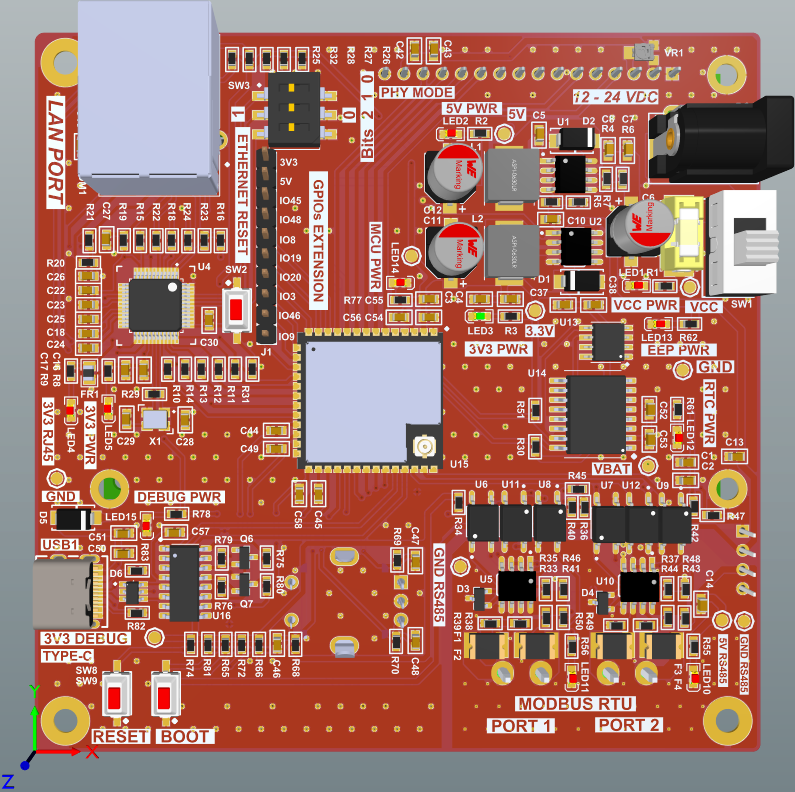
\includegraphics[width=\textwidth]{image/top_3d.png}
    \end{minipage}
    \hfill
    \begin{minipage}{0.48\textwidth}
        \centering
        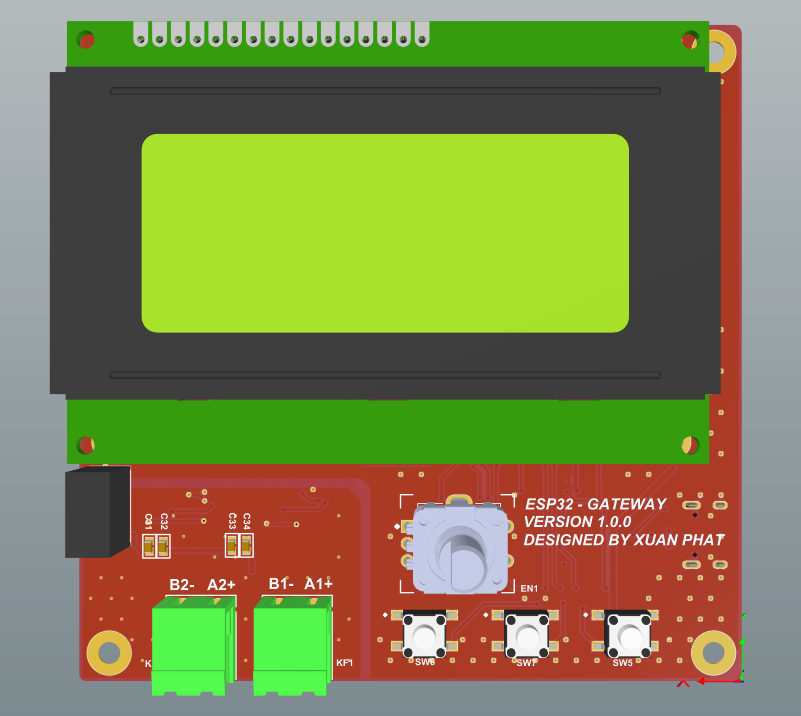
\includegraphics[width=\textwidth]{image/bottom_3d.png}
    \end{minipage}
    \caption{Hình ảnh mạch 3D khi đã đặt linh kiện của lớp Top và lớp Bottom}
    \label{fig:bottom_hide_3d}
\end{figure}

\begin{figure}[H]
    \centering
    \begin{minipage}{0.48\textwidth}
        \centering
        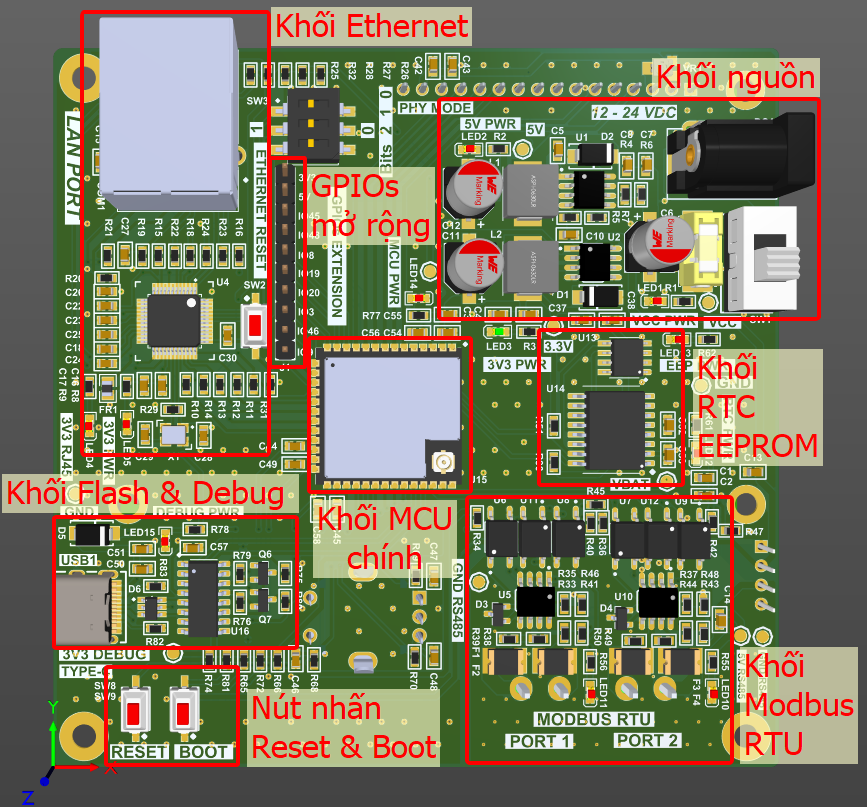
\includegraphics[width=\textwidth]{image/detail_board.png}
    \end{minipage}
    \hfill
    \begin{minipage}{0.48\textwidth}
        \centering
        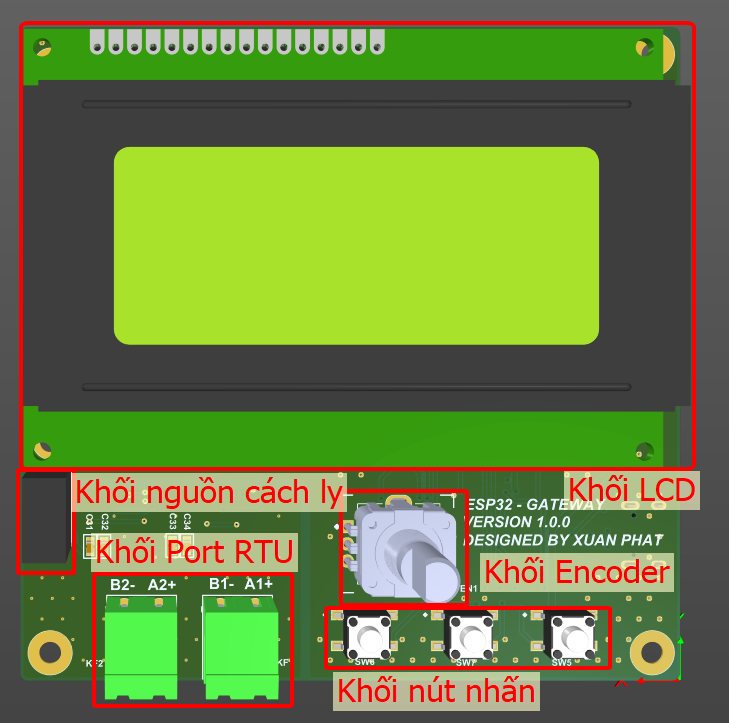
\includegraphics[width=\textwidth]{image/detail_board_bot.png}
    \end{minipage}
    \caption{Các khối chức năng trên mạch sau khi sắp xếp}
    \label{fig:bottom_hide_3d}
\end{figure}

\subsection{Thực hiện thi công mạch thực tế}
\begin{figure}[H]
    \centering
    \begin{minipage}{0.48\textwidth}
        \centering
        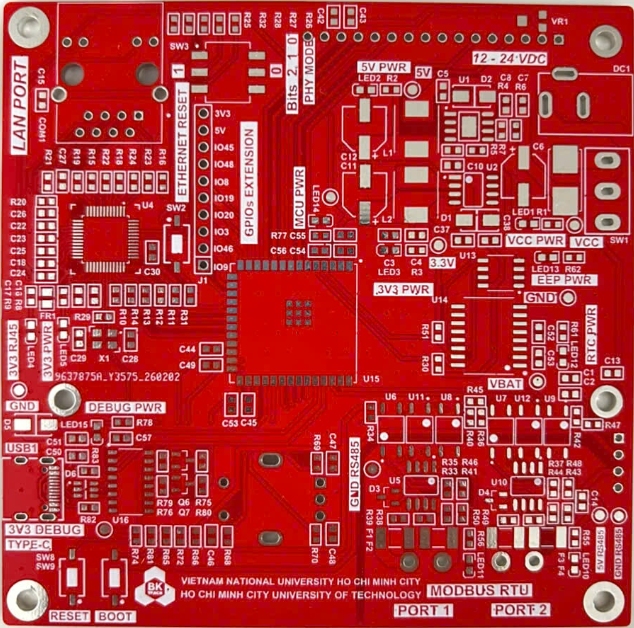
\includegraphics[width=\textwidth]{image/no_1.png}
    \end{minipage}
    \hfill
    \begin{minipage}{0.48\textwidth}
        \centering
        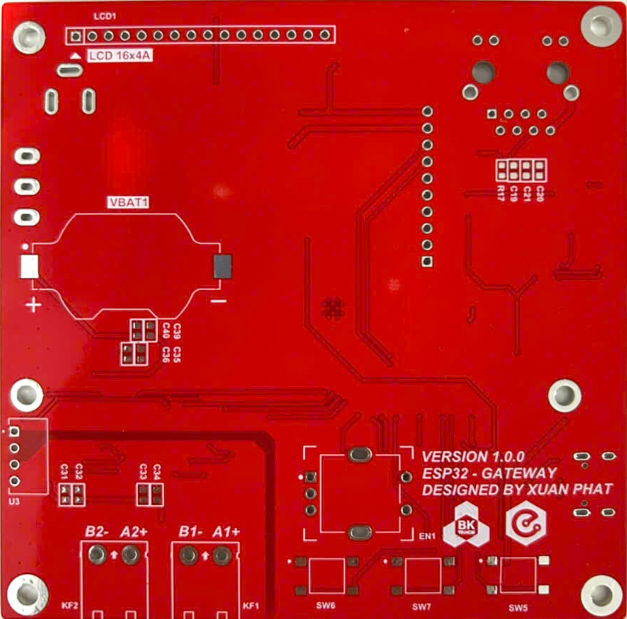
\includegraphics[width=\textwidth]{image/no_2.png}
    \end{minipage}
    \caption{Mạch khi chưa hàn linh kiện}
    \label{fig:bottom_hide_3d}
\end{figure}

\begin{figure}[H]
    \centering
    \begin{minipage}{0.48\textwidth}
        \centering
        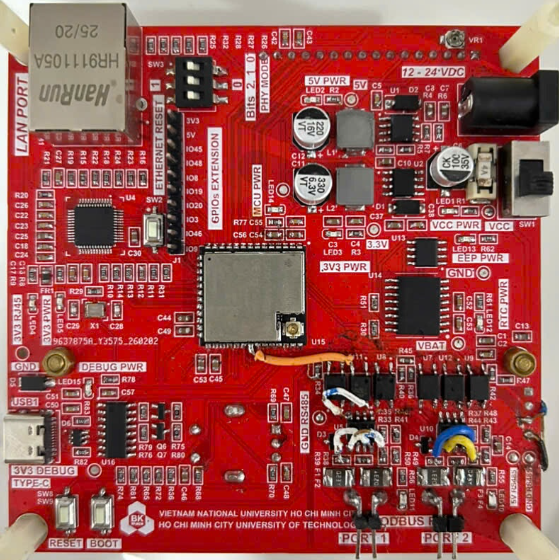
\includegraphics[width=\textwidth]{image/bot_board.png}
    \end{minipage}
    \hfill
    \begin{minipage}{0.48\textwidth}
        \centering
        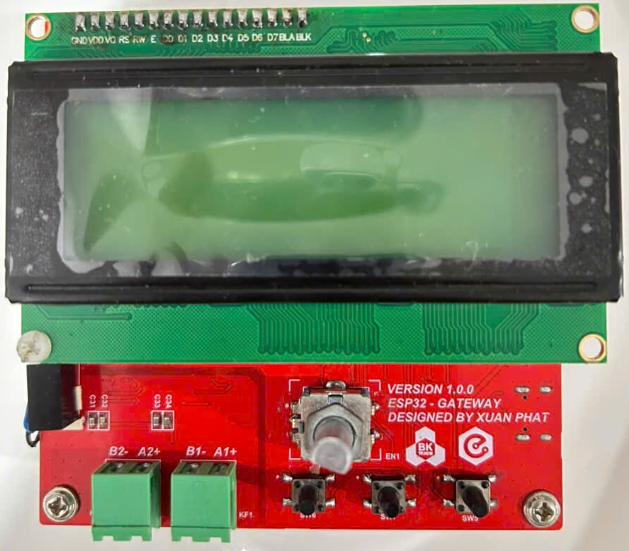
\includegraphics[width=\textwidth]{image/top_board.png}
    \end{minipage}
    \caption{Mạch sau khi đã hàn các linh kiện lên mạch}
    \label{fig:bottom_hide_3d}
\end{figure}

Mạch thực tế sau khi hàn các linh kiện và sửa các lỗi chưa được phát hiện khi vẽ schematic chi tiết.

\section{Kết quả phần mềm App nhập dữ liệu}
\begin{figure}[H]
    \centering
    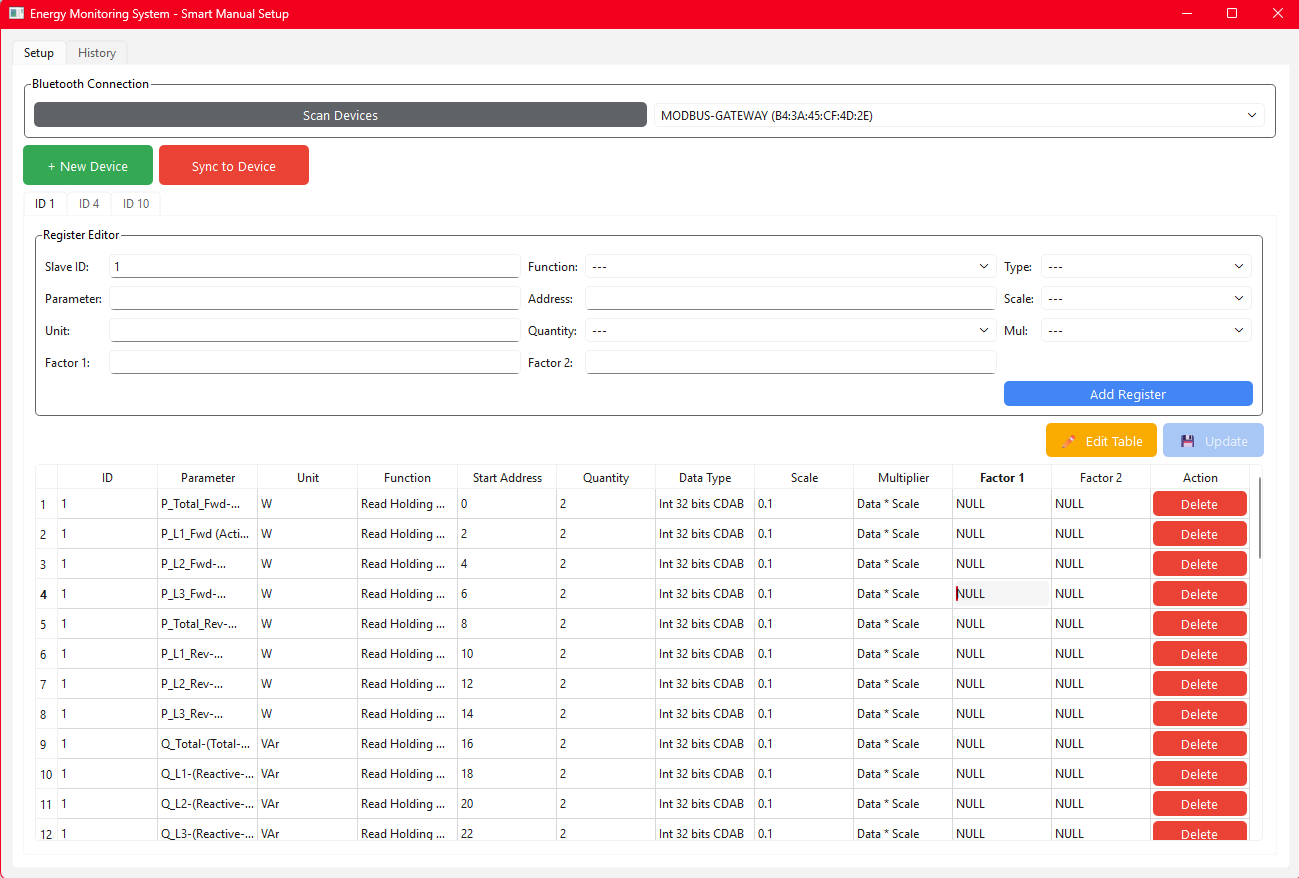
\includegraphics[width=1.1\textwidth]{image/tab_setup.png}
    \caption{Tab nhập liệu chính khi vừa khởi động App}
    \label{fig:add_new}
\end{figure}
\begin{figure}[H]
    \centering
    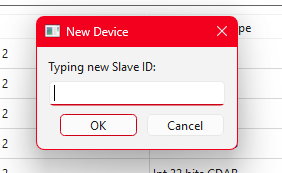
\includegraphics[width=0.4\textwidth]{image/add_new.png}
    \caption{Box nhập ID cho thiết bị mới}
    \label{fig:add_new}
\end{figure}
\begin{figure}[H]
    \centering
    \begin{minipage}{0.4\textwidth}
        \centering
        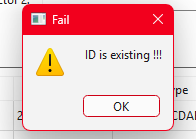
\includegraphics[width=\textwidth]{image/id_exist.png}
    \end{minipage}
    \hfill
    \begin{minipage}{0.4\textwidth}
        \centering
        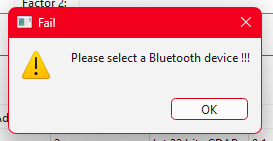
\includegraphics[width=\textwidth]{image/anno_no_device.png}
    \end{minipage}
    \caption{Thông báo lỗi khi ID đã tồn tại và thông báo lỗi khi chưa chọn thiết bị}
    \label{fig:bottom_hide_3d}
\end{figure}

\begin{figure}[H]
    \centering
    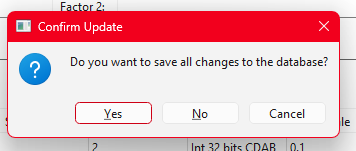
\includegraphics[width=0.4\textwidth]{image/update_confirm.png}
    \caption{Thông báo có cập nhật dữ liệu mới không}
    \label{fig:id_exist}
\end{figure}

\begin{figure}[H]
    \centering
    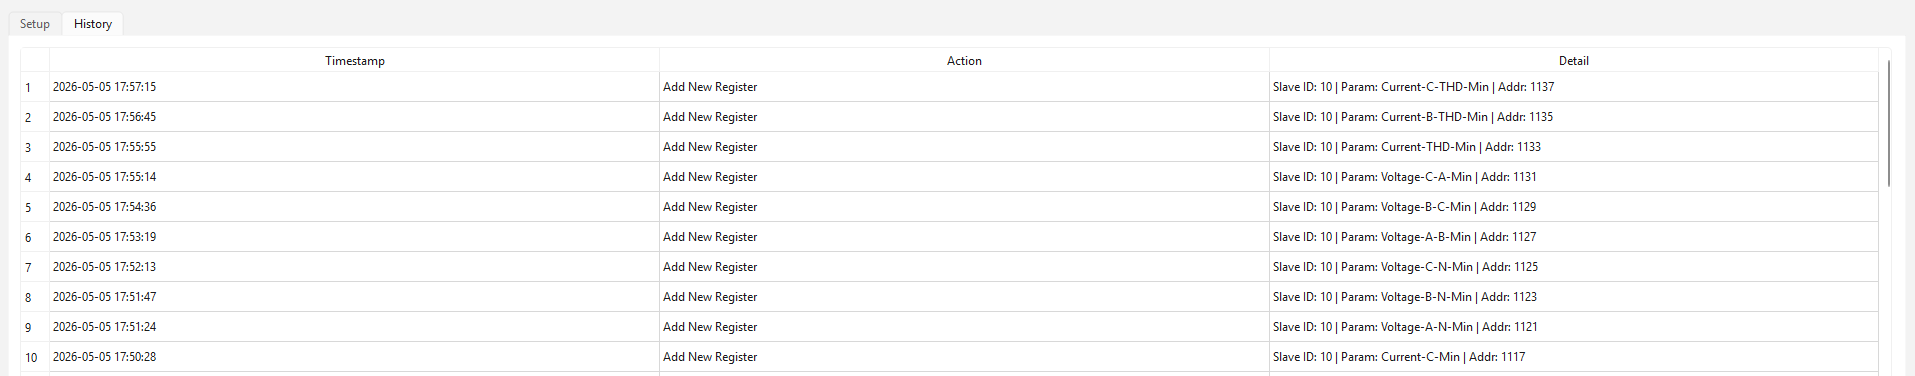
\includegraphics[width=1.1\textwidth]{image/tab_his.png}
    \caption{Tab lịch sử của App}
    \label{fig:add_new}
\end{figure}


\begin{figure}[H]
    \centering
    \begin{minipage}{0.9\textwidth}
        \centering
        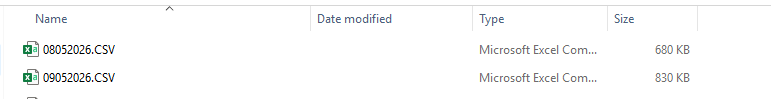
\includegraphics[width=\textwidth]{image/excel_1.png}
    \end{minipage}
    \hfill
    \begin{minipage}{0.9\textwidth}
        \centering
        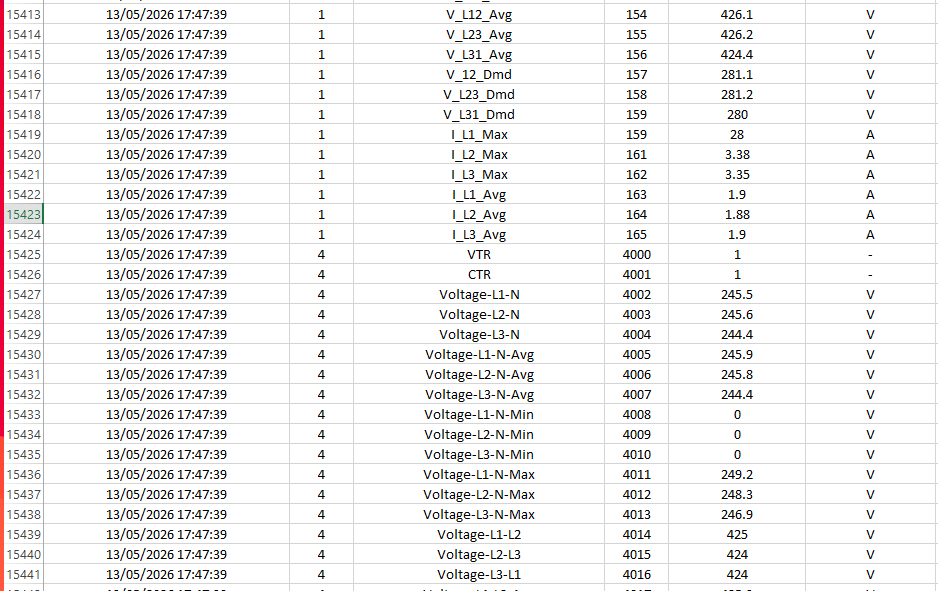
\includegraphics[width=\textwidth]{image/excel.png}
    \end{minipage}
    \caption{Lưu giữ liệu vào thẻ nhớ SD Card và lưu dữ liệu theo từng ngày}
    \label{fig:bottom_hide_3d}
\end{figure}
Thời gian được đọc từ RTC, thực hiện tạo tên file mới theo định dạng ngày tháng năm, so sánh với các tên file
hiện có trong thẻ nhớ, nếu đã tồn tại thì tiếp tục ghi vào các file cũ, nếu chưa có thì tạo một file mới với
tên file là ngày tháng năm.



\section{Kết quả phát triển giao diện Dashboard}

\begin{figure}[H]
    \centering
    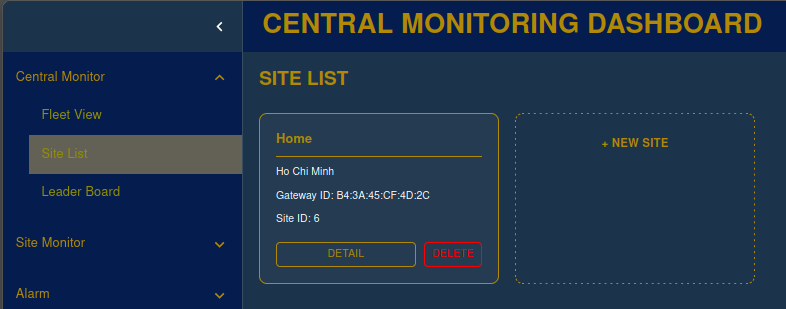
\includegraphics[width=0.9\textwidth]{image/site_list.png}
    \caption{Hiển thị các site có trong hệ thống của user}
    \label{fig:site_list}
\end{figure}

\begin{figure}[H]
    \centering
    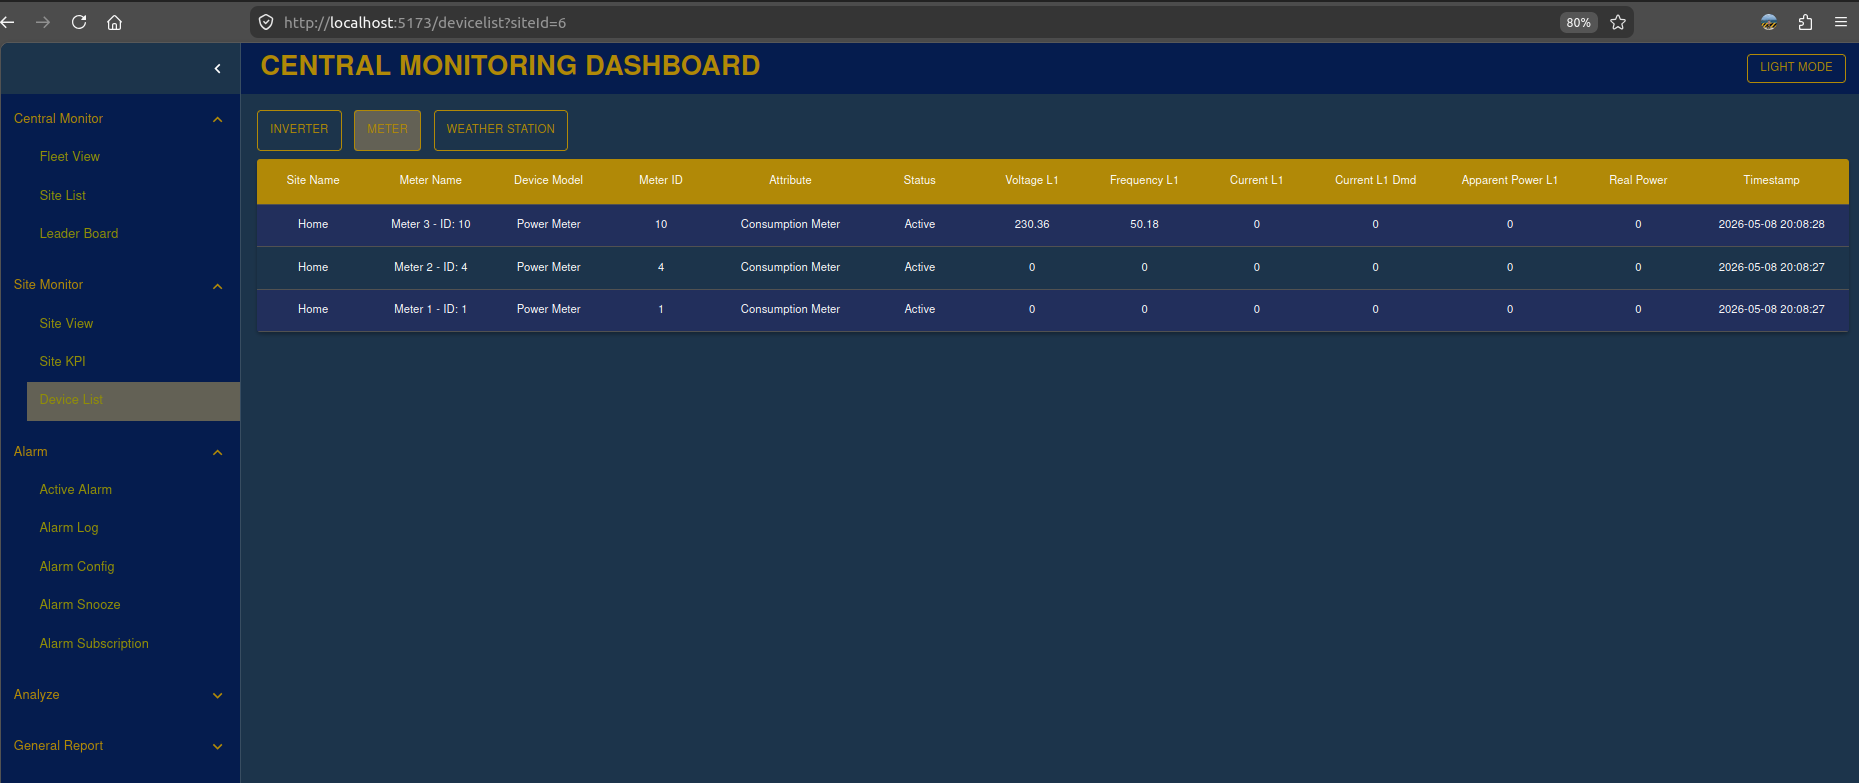
\includegraphics[width=0.9\textwidth]{image/device_list.png}
    \caption{Dữ liệu các đồng hồ điện hiển thị tổng quát trên trình duyệt web}
    \label{fig:deivce_list}
\end{figure}
Cung cấp hai nút nhấn giúp người dùng có thể xem được thông các đồng hồ điện bên trong site đó và nếu site đó không dùng thì có thể xóa hoàn toàn.
Trong đồ án này ta thực hiện gán một thiết bị thu thập dữ liệu cho một site thông qua dải ID có trên thiết bị khởi tạo.
\begin{figure}[H]
    \centering
    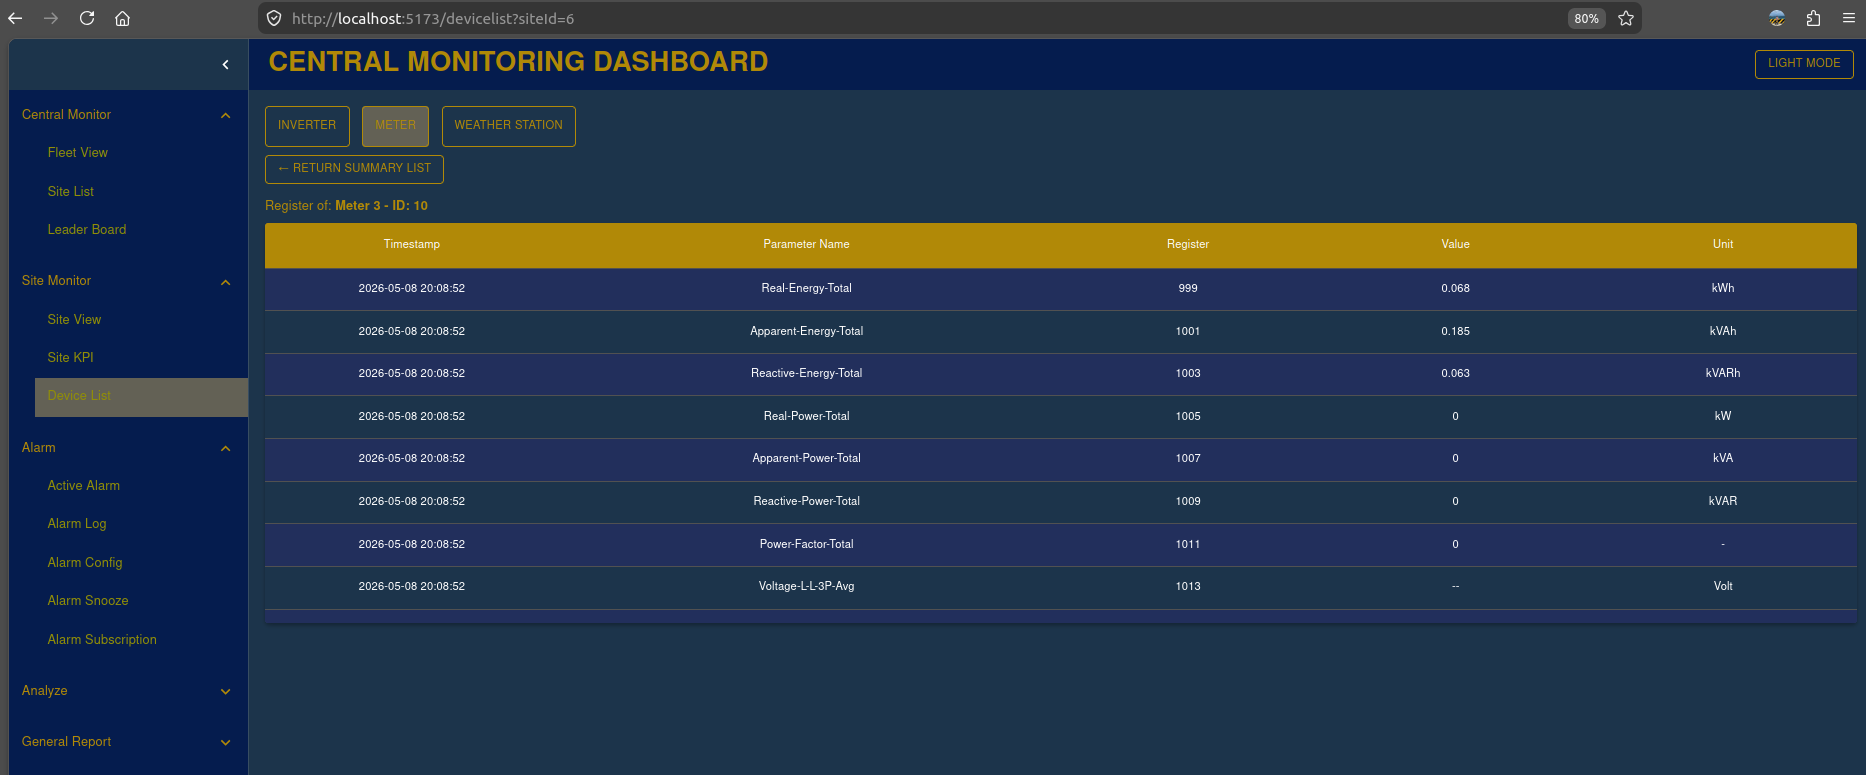
\includegraphics[width=0.9\textwidth]{image/detail_reg.png}
    \caption{Dữ liệu từng thanh ghi của từng đồng hồ điện}
    \label{fig:detail_reg}
\end{figure}
Khi người dùng nhấp vào dòng của một đồng hồ bất kì thì dữ liệu chi tiết của đồng hồ điện đó hiện ra từng thanh ghi.
Các thanh ghi nhập từ App sẽ xuất hiện toàn bộ trong trang này.

\begin{figure}[H]
    \centering
    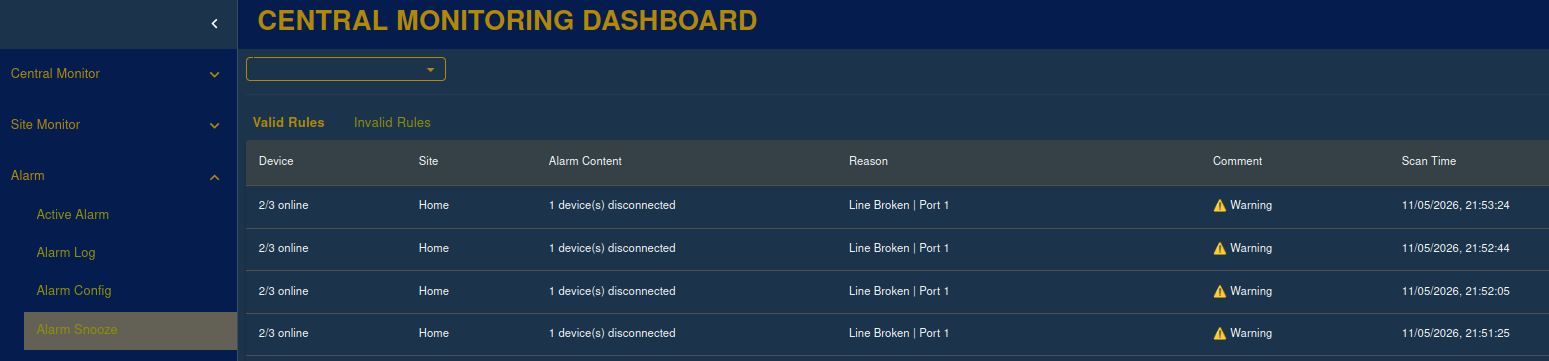
\includegraphics[width=1\textwidth]{image/alarm_table.png}
    \caption{Bảng tổng quát các cảnh báo đã gửi lên từ thiết bị}
    \label{fig:detail_reg}
\end{figure}
Tại đây các cảnh báo liên quan đến các sự cố đường truyền được thiết bị phát hiện trong quá trình thu thập dữ liệu hoặc phán hiện khi người dùng sử dụng
nút nhấn chức năng trên thiết bị để thực hiện kiểm tra đường trường.
Khi người dùng nhấp vào một cảnh báo bất kì thì trang web sẽ mô phỏng lại đường truyền kèm theo các lỗi cụ thể trên đường truyền tại thời điểm thiết bị gửi tin nhắn cảnh báo.
Backend của trang web tiến hành đăng ký nhận tin nhắn cảnh báo từ thiết bị và tiến hành chờ, dữ liệu sau khi nhận từ MQTT Broker sẽ được lưu vào database của 
trang web và được gửi dữ liệu lên frontend thông qua Websocket, frontend dựa trên dữ liệu nhận được thì sẽ tiến hành mô phỏng đường truyền.
\begin{figure}[H]
    \centering
    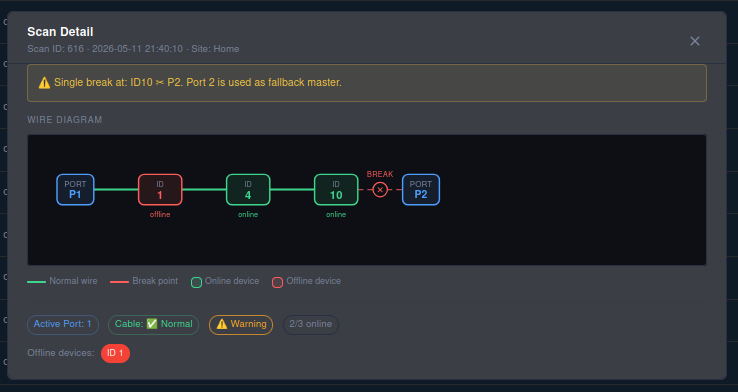
\includegraphics[width=0.9\textwidth]{image/detail_alarm.png}
    \caption{Hiển thị cụ thể thông tin đường truyền dựa trên Alarm gửi lên}
    \label{fig:detail_reg}
\end{figure}
Thực hiện mô phỏng lại đường truyền và các thiết bị hiện có trên đường truyền.
Quá trình khởi tạo hình ảnh mô phỏng được thực hiện bằng thư viện React ngay trên phần quản lý cảu Frontend.